\chapter{Design \& Implementation}\label{chap:design}
In this chapter we will discuss the development of the solution that was outlined in the previous chapter. The system will be explained in a top-down fashion, and as such we start off with an overview of the entire system through the architecture. Afterward, the specifics of each component will be explained in their own separate sections.

\section{Architecture}\label{sec:design_overview}
This system is built on an pipeline architecture, where the output of each primary component is fed into the next. The main benefit of this architecture is the modularity and scalability. Each component has minimal coupling with each other, by only interacting through data. As long as two components both adhere to the rules for data exchange, they can completely disregard any logic or functionality of each other. This gives the system the two advantageous properties of effortless exchange of entire components and straightforward horizontal scaling.

If system usage grows sufficiently large the data exchange could be handled by intermediate databases using, for example, a master-slave architecture where components supplying data could write to the database through one of multiple masters, and components retrieving data could read from one of multiple slaves. It is also possible to have every component run on different machines in different places. While this might not be a computational advantage, it minimizes logistics problems during scaling operations, since the system can be partially moved, component by component. Shutdown of a component can be delayed until its replacement is running. Regardless of the specific implementations, our usage of the pipeline architecture makes the system inherently modular and scalable. 

\subsection{Filtering and Refinement}
Since the potential input size of testing all possible combinations of articles for missing links is roughly 5 million articles squared, which totals to $2.5 \times 10^{13}$, we have employed a \emph{filtering and refinement} strategy. The filtering step chooses the more promising candidates based on a given policy, and the refinement step does the actual evaluation of the candidates.

\tikzsetnextfilename{system-overview}
\begin{figure}[tb]%
  \centering
  \begin{tikzpicture}[node distance = 2.84cm, auto]
    \node [database, yshift=1em] (db) {DB};
    \node [bigblock, right of=db] (ap) {Article Picker};
    \node [bigblock, right of=ap] (tfl) {Feature Extraction};
    \node [bigblock, right of=tfl] (classifier) {Classifier};
    \node [database, right of=classifier] (db2) {DB2};
    \node [bigblock, below=1cm of db2] (web) {Web Interface};
    
    %\node [above=1cm of ap] (inputarticle) {};
    
    \node [smallblock, below=1.5cm of ap, xshift=-2em] (n2v) {Node2Vec};
    \node [smallblock, below=.5cm of n2v] (paropt) {Parameter Optimizer};
    
    \node [smallblock, below=4.5cm of tfl] (prepper) {Training Data Generator};
    \node [smallblock, right of=prepper] (classifierTrainer) {Classifier Trainer};
    
    \begin{scope}[on background layer]
    \node [container, fit=(n2v)(paropt)] (container1) {};
    \node[below] at (container1.north) {Feature Learning};
    \node [container, fit=(prepper)(classifierTrainer)] (container2) {};
    \node[above] at (container2.south) {Classifier Model Learning};
    
    \node [container, fit=(db)(db2)] (container3) {};
    \node[below] at (container3.north) {Main Pipeline};
    \end{scope}
    
    %\draw [->] (db) -- (n2v);
    
    \path [line] (db) -- (ap);
    %\path [line] (inputarticle) -- (ap);
    \path [line] (ap) -- (tfl);
    \path [line] (tfl) -- (classifier);
    \path [line] (classifier) -- (db2);
    \path [line] (db2) -- (web);
    
    \path [line] (db.300) |- (n2v);
    %\path [line] (db.300) |- (paropt);
    \path [line] (db.240) |- (prepper);
    
    \path [line, swap, transform canvas={xshift=-1.3em}] (paropt) -- node{Parameters} (n2v);
    \path [line] (n2v.east) -| node [near end] {Model} ([xshift=-1.2em]tfl.south);
    
    \path [line] (prepper) -- (classifierTrainer);
    %\path [line] (prepper) -- (tfl);
    %\path [line] ([xshift=1.2em]tfl.south) -- ([xshift=1.2em]prepper.north);
    \draw [line] (prepper.north) |- ([xshift=1.2em, yshift=0.5em]tfl.south) -- ([xshift=1.2em]prepper.north);
    
    \path [line] (classifierTrainer) -- node{Model} (classifier);
    
  \end{tikzpicture}
\caption[Architecture diagram showing the major components of the system]{Architecture diagram showing the major components of the system. Each box is a component, and a dashed line box is a grouping of components. Arrows describe the way data flows.}%
\label{fig:system-overview}%
\end{figure}

\subsection{Main Pipeline}
The main pipeline consists of five components. The first one is a storage component, which holds all the information required to identify the link suggestions. The second component is \emph{Candidate Filtering}, which is responsible for the filtering process. As such, it extracts candidate article pairs from the database. The candidates are of the form $(A,B)$ where $A$ is a source article and $B$ is a suggested target article. The third component is the \emph{Feature Extractor}. This intermediate component generates a feature vector from a given candidate pair. As the fourth component we have the \emph{Classifier}, that is responsible for the refinement process. It does this by suggesting link that should be added to the input pair, based on the feature vector it received. Finally the \emph{Results Pool} is another storage component, which holds the suggestions until they are evaluated through the user interface.

\subsection{Model Training}
Construction of the main pipeline includes learning a model for extracting features from article, as well as training a classifier. These tasks are performed by two support modules.

The support module for the feature learning consists of a \emph{Model Trainer} and a \emph{Parameter Optimizer}. The \emph{Parameter Optimizer} works on a smaller subset of the dataset in order to speed up the process of tuning the parameters. When an acceptable set of parameters has been found, the \emph{Model Trainer} uses these parameters to train a model on the entire dataset. The result of this is the model, which is used as the \emph{Feature Extractor}.

The other support module is for the classifier learning process. It consists of a \emph{Training Data Generator} and a \emph{Classifier Trainer}. The \emph{Training Data Generator} retrieves training pairs and labels from the dataset, and uses the \emph{Feature Extractor} to prepare the data. Then the \emph{Classifier Trainer} uses this prepared training data to create a model, which is used as our classifier.

\subsection{User Interface}

Finally, we cover the User Interface. The purpose of this component is to publish the results of the main pipeline to users who can then use the results to edit Wikipedia. Since the classifier can not be expected to reach a perfect precision, the final decision of whether to include a suggested link, should be done by a human editor. Therefore we create a user interface that allows people to retrieve the results of the main pipeline.

We consider this component separate from the main pipeline. The reason is different requirements of the two parts. While both the user interface and the main pipeline share the goals of then entire system, they have different subgoals. The main pipeline is purely focused on producing results, and the user interface only considers the delivery of those results. This difference in subgoals requires a different evaluation approach, and as such it is valuable to separate the user interface from the main pipeline.

\section{Database}\label{sec:db}
Our approach to identifying missing links requires readily available data, which we facilitate by storing the required data in a local database. This database is the first component in the main pipeline seen in \cref{fig:system-overview}. 

\subsection{Database Design}\label{sec:db_design}
Because of the need to store a graph as mentioned in \cref{sec:choice_of_graph}, a natural choice is to use a native graph database. We use Neo4j~\cite{neo4j} as it performs well for graph based queries, and supports extensions to its query language through Java plugins. The data model in Neo4j is based on nodes, relationships between nodes, and properties on these. Each node and relationship can be annotated with labels to distinguish between types when querying the database.

We store Wikipedia articles as nodes with their title as a property, and links between articles as relationships. Labels are used to distinguish between types of articles and links.

\begin{table}[tbp]
  \centering
  
    \begin{tabular}{@{}p{.20\textwidth}p{.60\textwidth}@{}}
      \toprule
      \textbf{Label}         & \textbf{Description}                            \\ \midrule
      \mono{Article}                   & A Wikipedia article                             \\
      \mono{FeaturedArticle}           & A Wikipedia article marked as \emph{Featured}   \\
      \mono{GoodArticle}               & A Wikipedia article marked as \emph{Good}       \\
      \mono{RedirectPage}           & A redirecting Wikipedia page                    \\
      \bottomrule
    \end{tabular}
    \caption[Node labels in the database]{Node labels in the database}%
    \label{tab:db_labels_nodes}
\end{table}
\begin{table}[tbp]
    \centering
    \begin{tabular}{@{}p{.20\textwidth}p{.60\textwidth}@{}}
      \toprule
      \textbf{Label}         & \textbf{Description}                            \\ \midrule
      \mono{LinksTo}              & A link between two articles                     \\
      \mono{TrainingData}         & A link that can be used during training         \\
      \mono{TestData}             & A link that is used only during testing \\
      \mono{RedirectsTo}          & An edge describing a redirect                   \\ \bottomrule
    \end{tabular}
    \caption[Relationship labels in the database]{Relationship labels in the database}%
    \label{tab:db_labels_edges}
\end{table}

\subsection{Populating the Database}\label{sec:db_populate}
%Because Wikipedia requests that bots are not used to crawl the articles~\cite{wiki-bots}, we instead use a readily available dataset from DBpedia~\cite{dbpedia}. This dataset is just a dump of all Wikipedia \emph{pages}. The pages consists of for example articles, user pages, and talk pages. Since we are only interested in articles, we prune non-article pages based on the namespace prefixes used on Wikipedia.
Because Wikipedia requests that bots are not used to crawl the articles~\cite{wiki-bots}, we instead use readily available datasets\footnote{Data extracted from Wikipedia dumps in October 2015} from DBpedia~\cite{dbpedia}. The datasets used are a list of all page links and a list of page redirects. The pages consists of articles as well as pages for users, talks, files, etc. Since we are only interested in articles, we prune non-article pages based on the namespace prefixes used on Wikipedia.

Redirects are responsible for redirecting synonyms and common misspellings to the main article. For example, trying to access the article on ``Santa'' will redirect to ``Santa Claus''. The redirects are necessary to include since they are referred to by many links. We do not handle these redirects when creating the database. Instead we handle them by following them as needed when we later traverse the graph.

%To add relationships between the article nodes in the the database, we could have parsed the text in each article and created edges based on all encountered links. However, DBPedia have created a separate dataset containing links in an accessible tuple format:
%\begin{center}
%\mono{\emph{<source\_page> <type> <target\_page>}}
%\end{center}

%We therefore use this dataset instead of manually extracting the links.
We create nodes for all article and redirect pages and relationships for the links and redirects, with the labels seen in \cref{tab:db_labels_nodes,tab:db_labels_edges}. While importing the articles and links into the database, additional labels \mono{FeaturedArticle} and \mono{GoodArticle} are also added to  \emph{featured} and \emph{good} articles respectively.

As seen in \cref{tab:db_labels_edges}, the links are split into three groups, \mono{LinksTo}, \mono{TrainingData}, and \mono{TestData}, to later accommodate test and evaluation of the classifier. The split is made randomly, according to a partitioning given in \cref{sec:classifier}.

The counts for the labels in the populated database is shown in \cref{tab:db_counts_nodes,tab:db_counts_edges}.

%page_links_unredirected_en.ttl.bz2
%redirects.en.ttl.bz2

\begin{table}[tbp]
  \centering
  \begin{minipage}[t]{0.45\textwidth}
    \centering
    \begin{tabular}{@{}lr@{}}
      \toprule
      \textbf{Label}         & \textbf{Count}     \\
      \midrule
      \textit{Nodes (total)} & \textit{\num{18172630}}  \\
      \mono{Article}         & \num{11159213}           \\
      \mono{FeaturedArticle} & \num{4820}               \\
      \mono{GoodArticle}     & \num{23741}              \\
      \mono{RedirectPage}    & \num{7013417}            \\ \bottomrule
    \end{tabular}
    \caption[Counts for node labels]{Counts for node labels. Note that some nodes have multiple labels.}%
    \label{tab:db_counts_nodes}
  \end{minipage}
  \hfill
  \begin{minipage}[t]{0.45\textwidth}
    \centering
    \begin{tabular}{@{}lr@{}}
      \toprule
      \textbf{Label}         & \textbf{Count}     \\ \midrule
      \textit{Relationships (total)} & \textit{\num{145878042}} \\
      \mono{LINKS\_TO}               & \num{138422339}          \\
      \mono{TRAINING\_DATA}          & \num{294857}             \\
      \mono{TEST\_DATA}              & \num{147429}             \\
      \mono{REDIRECTS\_TO}           & \num{7013417}            \\ \bottomrule
    \end{tabular}
    \caption[Counts for relationship labels]{Counts for relationship labels.}%
    \label{tab:db_counts_edges}
  \end{minipage}

\end{table}


%\section{Detailed View of Components}\label{sec:detailed_view}
%\todo{Maybe each of the following subsections should be their own section. As it is now, we go pretty deep into subsubsection! This probably depends on how brief/long each component will be.}

%Here, we will describe each component individually. \todo{Refer to \cref{fig:system-overview}}

\section{Candidate Generator}
The candidate generator component is responsible for providing an ordering of article pairs that are to be classified. The motivation behind this component and how we choose candidate pairs is described in this section.

The database contains roughly 11 million articles, which results in $1.21 \times 10^{14}$ article pairs, making a brute force approach that randomly generates all article pair permutations infeasible. Considering that the highest number of links on an article is currently 7130\footnote{The article in question is \enquote{List of Places In Afghanistan}}, and that the brute force approach checks 11 million potential links, it is safe to assume that most of these article pairs should not be linked.

Therefore we want a more efficient selection method, that seeks to order the article pairs, such that that should be linked, will generally be evaluated in the pipeline before those that should not. The candidate generator attempts to solve this task of efficiently selecting pairs. A perfect ordering method would result in having all the article pairs that should be linked, occur before any article pair that should not be linked. While such a method would be helpful, it is unrealistic and only serves as a benchmark.

Instead of aspiring to create a perfect method, we only require the method to be a heuristic that performs reasonably well, generating enough candidate pairs for providing a sufficient number of link suggestions. The problem here is that in order to evaluate the exact performance of a policy, we would need to know if the candidate pairs it suggests, will be classified mostly as positive. Because such an evaluation of the candidate generator would produce the results of the classifier, it would in turn make the method obsolete for the tested pairs, since they would now have been classified. \todo{ikke den fede formulering. Lad dog vær med at bruge tid på dette før til aller sidst. Andre ting er vigtigere} Therefore we choose our method mainly from a combination of intuition and preliminary tests.

Our chosen method is a combination of two approaches. One is based on a \emph{clickstream} dataset and the other on a simple textual analysis.

\subsection{Clickstream Approach}\label{sec:candidate_clickstream}

The clickstream approach is inspired by related work that uses server logs to predict missing links~\cite{hyperlink-structure-using-logs}. We use clickstream~\cite{wiki-clickstream} data built from Wikipedia server logs, and as such it is based on user behavior. A clickstream data source is a list of requests that Wikipedia received within a given timespan\footnote{We use a data source collected from March 1 -- March 31, 2016}. A request holds information on a referrer and a resource, as well as a count of the occurrence of this request and a request type. The request type can be \emph{link}, \emph{external}, or \emph{other}. For this approach, the type \emph{other} is the only relevant one. A request of type \emph{other} means that the referrer and resource were both Wikipedia articles, but that referrer does not link to the resource. One source of this type of requests could be searches~\cite{wiki-clickstream}.

The heuristic for this approach, is that some of these requests will indicate that a user, after reading one article, was prompted to read another article, and that they did not have the possibility of following a link. While there are plenty of cases where this does not constitute a missing link, chances are that some of the requests are examples of this. The approach iterates through the clickstream data, picking out requests of type \emph{other}, and ranking them by their number of occurrences.

Though preliminary results with this approach have been promising, it produces a limited amount of candidate pairs (1.7 million). Therefore, we choose to complement it with another approach to get a bigger set of candidate pairs.

\subsection{n-gram Approach}

For the complementary approach we took inspiration from~\cite{milne2008learning}, where they employ textual analysis to find article pairs. The inspiration lies in their use of n-grams to find article pairs. For each article we create a set of shingles from an n-gram search. We then search through the titles of Wikipedia articles, for ones that are contained in at least one of the shingles. This gives us a large set of article pairs $(a,b)$, where article $a$ mentions article $b$.

However, this is a crude approach and a significant amount of the candidate pairs can easily be discarded. Consider the Wikipedia article on the word \enquote{the}. With the n-gram approach, nearly all encyclopedia articles would be in a candidate pair with this article, where only a fraction would be worth considering.

%A way to combat this would be to order the candidate pairs according to the inverse frequency of target articles. The intuition is that articles, which are rarely mentioned across all articles, will be more significant when they \emph{are} mentioned. It is likely that a frequency threshold will be required, since the advantages of the approach becomes negligible at some sufficiently high frequency.
\todo{Vi har slettet noget om inverse document frequency, er det okay?}

Another considerable problem with the approach is that while it does provide many candidate pairs, it can not be guaranteed to order all possible pairs, and therefore it will not completely cover the complement of the clickstream approach. A preliminary test with a 5-gram search through featured articles gave us more than a million candidate pairs. When all articles are searched, this approach will generate significantly more than the clickstream approach. This will be sufficient for our usage, and further scaling will not be implemented in this project.

%from an article $a$ to an article $b$ in the time frame where the data was collected, as well as the method of navigation of these clicks. One of these methods of navigation is a \emph{teleportation}, which means the user ended up on article $b$ after having viewed article $a$, but not following a link.

%By selecting article pairs without an existing link and that users have navigated between by teleportation, the articles might be related and inserting a link between the articles might improve navigability.



\section{Feature Extractor}\label{feature_extractor}
The next component in the main pipeline is the feature extractor. This component generates the feature representation of a candidate pair as described by the function $f$ in \cref{sec:ml_def}, which can then be used for classification.

The feature extractor returns a single feature vector, representing the link between a given source and target article pair. As we need to classify both existing and non-existing links, it must be possible to extract feature vectors in both cases. Therefore the feature vector for a link is constructed by combining the feature vectors of the source and target articles.

As mentioned in \cref{sec:feature_generation} we aim to use feature learning, specifically network embedding, to learn these feature representations. While there are several different ways to approach network embedding, we found node2vec~\cite{node2vec} to be suitable. The main advantage of node2vec is increased flexibility compared to other well-known approaches due to tunable hyperparameters~\cite{node2vec}, which allows us to experiment with different neighborhood exploration methods Additionally, node2vec offers highly competitive performance, and performs well for large networks~\cite{node2vec}.

This section describes how node2vec is used to generate the feature representation, along with the process of optimizing the models hyperparameters.

\subsection{Description of node2vec}
\label{sec:node2vec}
node2vec is an algorithmic framework for semi-supervised feature learning in networks~\cite{node2vec}. The goal of the algorithm is to learn feature representations for nodes in a network. To find feature representations for edges, the feature representation for two nodes can be combined. The node2vec paper proposes a way of generating features representations for nodes based on their neighborhoods. The idea is to use word embedding, where nodes are used as words, and node sequences are used as sentences. The neighborhood of a node consists of the nodes that are close in the node sequence. In the following sections we briefly describe word embedding, and how node sequences are constructed using biased random walks in the graph. Furthermore we describe the approaches to combine node vectors presented in \cite{node2vec}, and propose a new combination method tailored for this project.

\subsubsection{Word Embedding}
Using nodes as words and node sequences generated by biased random walks as sentences allows the use of word embedding algorithms on the sentences, mapping words to vectors. The node2vec reference implementation uses a well-known model for word embedding called word2vec. Intuitively, two words are related if they are close to each other in a sentence. A parameter $k$ specifies the size of a context window that defines the number of surrounding words that should be considered in the same context. In node2vec the context window is used for sampling neighborhoods of nodes, where it determines the size of the neighborhood.

\subsubsection{Neighborhoods}
The notion of neighborhoods is important in network embedding, as the features of a node is derived from its neighborhood. Intuitively, this implies similarity between nodes that have similar neighborhoods. The neighborhood of a given node is found by traversing the graph.

In node2vec the neighborhoods of each node $n$ is found by performing a series of biased random walks, and then observing the $k$ nearest nodes on either side of $n$ in the walks. To ensure that all nodes are visited during the random walks a number of walks, specified by the $r$ parameter, are started in every node. The maximum length of each walk is specified by the $l$ parameter.

The random walks are biased using two parameters, $p$ and $q$. An example of the biased random walk is shown in \cref{fig:randomwalk}. The walk is currently in $v$, after walking the edge $(t,v)$. Here a search bias $\alpha$ is given to each outgoing edge from $v$ according to \cref{eq:bias}, where $d_{tx}$ denotes the shortest distance from $t$ to $x$. The next edge in the walk is selected by probability sampling using the alias method.

\begin{equation}
\label{eq:bias}
\alpha_{pq}(t,x)=
\begin{cases}
  \frac{1}{p} & \text{if } d_{tx}=0 \\
  1           & \text{if } d_{tx}=1 \\
  \frac{1}{q} & \text{if } d_{tx}=2
\end{cases}
\end{equation}

By adjusting $p$ and $q$ it is possible to approximate different search strategies. A high $p$ value, relative to $\max(1,q)$, approximates a depth-first search, while a high $q$ value, relative to $\max(1,p)$, approximates the behavior of a breath-first search. The motivation for tuning these parameters is the observation that real-world networks can be structured in many ways. The biased random walks with the tunable $p$ and $q$ values accounts for different types of networks, by allowing control of the exploration method.

\begin{figure}%
  \centering
  \tikzsetnextfilename{nodewalk}
  \begin{tikzpicture}[node distance = 1.7cm, auto]
      \node [node] (v) {$v$};
      \node [node, fill=none, above left=of v,
              pin={[pin distance=1.2em,pin edge={very thick}]15:},
              pin={[pin distance=1.2em,pin edge={very thick}]150:},
              pin={[pin distance=1.2em,pin edge={very thick}]230:}
              ] (x1) {$x_1$};
      \node [node, fill=none, above right=of v,
              pin={[pin distance=1.2em,pin edge={very thick}]350:},
              pin={[pin distance=1.2em,pin edge={very thick}]295:},
              pin={[pin distance=1.2em,pin edge={very thick}]150:}
              ] (x2) {$x_2$};
      \node [node, fill=none, below left=of v,
              pin={[pin distance=1.2em,pin edge={very thick}]170:},
              pin={[pin distance=1.2em,pin edge={very thick}]210:}
              ] (t) {$t$};
      \node [node, fill=none, below right=of v,
              pin={[pin distance=1.2em,pin edge={very thick}]330:},
              pin={[pin distance=1.2em,pin edge={very thick}]20:}
              ] (x3) {$x_3$};
      \path [draw, very thick, inner sep=.5pt] (x1) -- node [] {$\alpha = 1$} (v);
      \path [draw, very thick, inner sep=.5pt] (x2) -- node [] {$\alpha = 1/q$} (v);
      \path [draw, very thick, swap, inner sep=.5pt] (x3) -- node [] {$\alpha = 1/q$} (v);
      \path [draw, very thick] (t) -- (x1);
      \path [draw, very thick, swap, inner sep=.5pt] (t) -- node [] {$\alpha = 1/p$} (v);
  \end{tikzpicture}
\caption[Illustration of random walk in node2vec]{Illustration of the random walk procedure in node2vec. The walk is currently in $v$ and came from $t$. It is now evaluating its next step out of node $v$. Adapted from~\cite{node2vec}.}%
\label{fig:randomwalk}%
\end{figure}

\subsubsection{Combining Feature Vectors}
By training a node2vec model on the graph, we are able to learn a function $h:V \to \mathbb{R}^d$, mapping a vertex to a vector representation of features. In order to construct a feature representation of a potential edge between two vertices, we need to combine their feature vectors. In the node2vec paper~\cite{node2vec} four different binary operators $\circ : \mathbb{R}^d \times \mathbb{R}^d \to \mathbb{R}^d$ for combining two feature vectors are examined, with \emph{Hadamard product} yielding the best results in all tested cases.

%We discovered that all 4 operators where commutative meaning that $a \circ b = b \circ a \ \forall a,b \in \mathbb{R}^d$ which works well in undirected graphs.

All of the four operations are commutative, which is suitable for undirected graphs, where the combined result vector does not depend on the order of the vertices. For directed graphs however, the order is important.

%If we have 2 pairs of articles $(a,b) \in \Rightarrow$ and $(b,a) \in V \times V \setminus \Rightarrow$ they will have the same feature representation using any of these 4 operators, but different labels.

If we are given two article pairs $(a,b)$ and $(b,a)$ where $a \Rightarrow b$ and $b \not \Rightarrow a$, their feature representations should intuitively be different because they have different labels.

%For this reason we will test different non-commutative operations.

Because Hadamard product produced good results in the node2vec paper we will be testing it and compare it to the corresponding non-commutative operation Hadamard division. Furthermore we choose to test concatenating the feature vectors $\mathbb{R}^d \times \mathbb{R}^d \to \mathbb{R}^{2d}$, leaving it up to the classifier to interpret the combination of article features.

% \section{Overview of node2vec} % (fold)
% \label{sec:overview_of_node2vec}

% Node2vec is an algorithmic framework for semi-supervised feature learning in networks~\cite{node2vec}. The goal of the algorithm is to learn a model that can reconstruct the neighborhood of a given node.

% The neighborhoods of each node is constructed by performing a number of biased random walks. The walks are biased using two parameters $p$ and $q$. A high $p$ value, relative to $max(1,q)$, approximates a depth-first search, while a high $q$ value, relative to $max(1,p)$, approximates the behavior of a breath-first search. The motivation of these tunable parameters is the observation that real-world networks can be structured in many ways. The randomness and the tunable $p$ and $q$ values accounts for different types of networks, by allowing control of the exploration method.

% Using nodes as words and the random walks as sentences allows using word embedding algorithms on the sentences, mapping words to vectors of real numbers. The node2vec reference implementation uses word2vec for word embedding. Intuitively, if two words are close two each other in the sentence, they are related. The tunable parameter $k$ specifies the size of a context window that defines the number of surrounding words that should be considered in the same context. In node2vec the context window is used for sampling neighborhoods of nodes, where it determines the size of the neighborhood.

% There are three additional parameters in node2vec, $d$, $r$, and $l$, which determines the dimensions of the resulting feature vector, the number of random walks performed per node, and the maximum length of each walk, respectively.

% By training a node2vec model on the graph, we are able to learn feature representations for each node. However, we need to combine these features in order to construct a feature representation of a potential edge between the two nodes. We combine these two node feature vectors by using the Hadamard product, as this was found to give the best results in~\cite{node2vec}.
% section overview_of_node2vec (end)

% \tikzsetnextfilename{n2vbowtie}
% \begin{figure}[tbp]%
%   \centering
%     \begin{tikzpicture}[node distance = .9ex, auto, remember picture]
    \tikzstyle{n2vcontainer} = [rectangle, draw, inner sep=.5ex, fill=clshade]
    \tikzstyle{n2vc} = [thick, circle, draw, fill=clnode, text width=1.5ex, text centered, minimum height=1.5ex, inner sep=0pt]
    
    % LEFT SIDE (INPUT LAYER)
    \node [n2vc, label=left:{$x_1$}] (c1) {};
    \node [n2vc, below=of c1, label=left:{$x_2$}] (c2) {};
    \node [n2vc, below=of c2, label=left:{$x_3$}] (c3) {};
    \node [n2vc, below=of c3, draw=none, fill=none] (c3-h) {};
    \node [n2vc, below=of c3-h, label=left:{$x_k$}] (c4) {};
    \node at ($(c3)!.5!(c4)$) {$\vphantom{\int^0}\smash[t]{\vdots}$};
    \node [n2vc, below=of c4, draw=none, fill=none] (c4-h) {};
    \node [n2vc, below=of c4-h, draw=none, fill=none] (c4-hh) {};
    \node [n2vc, below=of c4-hh, label=left:{$x_V$}] (c5) {};
    \node at ($(c4)!.5!(c5)$) {$\vphantom{\int^0}\smash[t]{\vdots}$};
    % Gray background box:
    \begin{scope}[on background layer]
      \node [n2vcontainer, fit=(c1)(c5)] (inputcontainer) {};
      \node[above] at (inputcontainer.north) {Input layer};
    \end{scope}
    
    % RIGHT SIDE (OUTPUT LAYER)
    \node [n2vc, right=8.5cm of c1,label=right:{$y_1$}] (o1) {};
    \node [n2vc, below=of o1, label=right:{$y_2$}] (o2) {};
    \node [n2vc, below=of o2, label=right:{$y_3$}] (o3) {};
    \node [n2vc, below=of o3, draw=none, fill=none] (o3-h) {};
    \node [n2vc, below=of o3-h, label=right:{$y_j$}] (o4) {};
    \node at ($(o3)!.5!(o4)$) {$\vphantom{\int^0}\smash[t]{\vdots}$};
    \node [n2vc, below=of o4, draw=none, fill=none] (o4-h) {};
    \node [n2vc, below=of o4-h, draw=none, fill=none] (o4-hh) {};
    \node [n2vc, below=of o4-hh, label=right:{$y_V$}] (o5) {};
    \node at ($(o4)!.5!(o5)$) {$\vphantom{\int^0}\smash[t]{\vdots}$};
    % Gray background box:
    \begin{scope}[on background layer]
      \node [n2vcontainer, fit=(o1)(o5)] (outputcontainer) {};
      \node[above] at (outputcontainer.north) {Output layer};
    \end{scope}
    
    % MIDDLE (HIDDEN LAYER)
    \begin{scope}[xshift=4.4cm, node distance = .7ex]
    %\node [draw] at ($(inputcontainer)!.5!(outputcontainer)$) {
    %  \begin{tikzpicture}[remember picture]
            \node [n2vc, yshift=-1.5em, label=right:{$h_1$}] (h1) {};
            \node [n2vc, below=of h1, label=right:{$h_2$}] (h2) {};
            \node [n2vc, below=of h2, draw=none, fill=none] (h3-h) {};
            \node [n2vc, below=of h3-h, label=right:{$h_i$}] (h4) {};
            \node at ($(h2)!.5!(h4)$) {$\vphantom{\int^0}\smash[t]{\vdots}$};
            \node [n2vc, below=of h4, draw=none, fill=none] (h4-h) {};
            \node [n2vc, below=of h4-h, label=right:{$h_N$}] (h5) {};
            \node at ($(h4)!.5!(h5)$) {$\vphantom{\int^0}\smash[t]{\vdots}$};
            % Gray background box:
            \begin{scope}[on background layer]
              \node [n2vcontainer, fit=(h1)(h5)] (hiddencontainer) {};
              \node[above, yshift=1.5em] at (hiddencontainer.north) {Hidden layer};
            \end{scope}
    %    \end{tikzpicture}
    %};
    \end{scope}
    
    % LINES MAKING THE BOW TIE
    \draw (inputcontainer.north east) -- (hiddencontainer.north west);
    \draw (inputcontainer.south east) -- (hiddencontainer.south west);
    \draw (outputcontainer.north west) -- (hiddencontainer.north east);
    \draw (outputcontainer.south west) -- (hiddencontainer.south east);
    
    % The math stuff with the arrows 1
    \node at ($(inputcontainer)!.5!(hiddencontainer)$) {
      \begin{tikzpicture}[remember picture, node distance = 1ex]
        \draw [line] (0,0) -- (1,.5);
        \draw [line] (0,.5) -- (1,0);
        %\node [fit=(o1)(o5)] (outputcontainer) {};
        \node [below=1em of {(0.5,0)}] {$\mathbf{W}_{V\times N}=\{w_{ki}\}$};
      \end{tikzpicture}
    };
    
    % The math stuff with the arrows 2
    \node at ($(hiddencontainer)!.5!(outputcontainer)$) {
      \begin{tikzpicture}[remember picture, node distance = 1ex]
        \draw [line] (0,0) -- (1,.5);
        \draw [line] (0,.5) -- (1,0);
        %\node [fit=(o1)(o5)] (outputcontainer) {};
        \node [below=1em of {(0.5,0)}] {$\mathbf{W'}_{V\times N}=\{w'_{ij}\}$};
      \end{tikzpicture}
    };
    
  \end{tikzpicture}

% \caption[short desc]{Text. Adapted from \cite{word2vec-param-learning}}%
% \label{fig:n2v-figure}%
% \end{figure}

\subsection{Performance \& Scalability}
As also detailed in~\cite{node2vec}, node2vec is able to scale well. Every walk is independent from each other which means that many walks can take place in parallel; it is embarrassingly parallel. Our test machine has 16 CPU cores which we want to utilize. We therefore spawn 16 threads, each walking the graph. This allows full utilization of every CPU core.

As all walks have to be stored for the word2vec phase, we are concerned that the memory footprint of storing all walks in memory is too high. We therefore dump the walks to a file, and later stream this file into memory when training word2vec. \emph{Gensim}, the implementation of word2vec we use, is also able to fully utilize the CPU when training word2vec on the walks.

\subsection{Hyperparameter Optimization}\label{sec:hyperopt}
As described in \cref{sec:node2vec}, node2vec has many tunable hyperparameters. An overview of these can be seen in \cref{tab:node2vecparams}. In addition to the hyperparameters we will also examine the performance of different binary operations for combining node feature vectors. To find the parameters that give the best feature representation, we do a hyperparameter optimization pass. We first specify the parameter space that should be searched in. As this is a large space, it is not feasible to exhaust all possibilities. We therefore use the tool called Spearmint~\cite{snoek2012practical}, which performs Bayesian optimization by maximizing the expected improvement, to efficiently search for parameters that will minimize an objective function. The objective function is $1 - \text{F-score}$, where the F-score is found by running a classifier on the node2vec model learned from the parameters. By keeping the classifier and its parameters constant, we can find the best set of parameters by finding the lowest objective function value.

\begin{table}[tbp]
\centering
\begin{tabular}{@{}lp{.75\textwidth}@{}}
\toprule
\textbf{Parameter} & \textbf{Description} \\
\midrule
$p$          &   Return parameter that controls the likelihood of immediately revisiting the previous node in the walk~\cite{node2vec}.   \\
$q$          &   Controls to which degree the walk prefers to stay in the neighborhood or to explore outwards.   \\
$d$          &   The dimensionality of the learned features.   \\
$r$          &   The number of random walks per node.   \\
$k$          &   The size of the context window.   \\
$l$          &   The max length of the random walk.   \\
function     &   The function to use for combining node features, it can be hadamard product, hadamard divide or concatenate.   \\
\bottomrule
\end{tabular}
\caption[Description of parameters in node2vec]{Description of the various parameters in node2vec}%
\label{tab:node2vecparams}
\end{table}


%\todo{Beskriv at vi optimere på et sub sæt af graphen og at det er pga speed up.}
%\todo{del mængden er featured => good og det er fordi at så behøver vi ikke lave features for all noder men kun featured og good.}
In order to run a sufficient amount of parameter experiments within a reasonable timespan, we speed up each iteration of the optimization.
This is done by limiting node2vec to only consider a subset of the graph, as well as constraining the set of nodes a walk can start from. The subset consists of the set of featured and good articles, and the set of start nodes is featured articles. By doing this, features are only generated for featured and good articles, which greatly improves performance and still makes the algorithm able to walk several nodes because these types of articles can be expected to be reasonably linked. Due to this limitation it is only possible to find features for featured and good articles, this means that we can only run parameter experiments on the subset $\{(a,b) \in P \cup N \mid \text{b is good}\}$ of our training data.

%To speed up each iteration of the optimization, we limit the set of start nodes to featured articles.
The parameter optimization is entirely autonomous and the process should be able to optimize the the parameters automatically. This means that one can learn on graph networks without knowing the underlying graph structure.

We start with a coarse search to find a good range for some parameters. This is done with large grained values for each parameter that would show local optima. After this, we search a second time with finer grained values to further refine the local optima. After completing 83 experiments the objective function seemed to have converged, as shown on \cref{fig:spearmint}. The best parameters found are shown in~\cref{tab:paramopt_goodvalues}.

\begin{figure}%
  \centering
  \tikzsetnextfilename{spearmint}
  \begin{tikzpicture}
    \begin{axis}[
      scale only axis,
      height=5cm,
      width=0.9\textwidth,
      xmin=0, xmax=90,
      ymin=0, ymax=1,
      legend entries={Unsorted, Sorted},
      legend pos=north east,
      legend style={draw=none},
      xlabel={Iteration},
      ylabel={Score}
    ]
      \addplot[mark=square*, color=color4!30!white] table [x=x, y=y, col sep=semicolon] {chapter_design/unsorted.csv};

      \addplot[
        scatter,
        color=color2,
        scatter src=explicit symbolic,
        scatter/classes={
            normal={mark=*, color2},%
            special={mark=*, colorG, draw=colorGshade}%
        }%,
        %pins near some coords={15/south:Hadamard,29/north:Divide}
      ] table [x=x, y=y, col sep=semicolon, meta=color] {chapter_design/sorted.csv}
      ;
      \node[coordinate,pin={[pin distance=1cm]above:{Hadamard}}]
        at (axis cs:16,0.55340945711058)	{};

      \node[coordinate,pin={[pin distance=.6cm]below:{Divide}}]
        at (axis cs:30,0.4252592596720848)	{};

      \node[coordinate,pin=above:{Concatenate}]
        at (axis cs:84,0.19147061365923185)	{};

    \end{axis}
  \end{tikzpicture}
\caption[Hyperparameter optimization]{Graph showing the progress of the hyperparameter optimization process}%
\label{fig:spearmint}%
\end{figure}

\begin{table}%
\centering
\begin{tabular}{ccccc}
\toprule
$p$  & $q$     & $d$ & $k$ & $l$ \\
\num{0.50} & \num{100000} & 256 & 80  & 80 \\
\bottomrule
\end{tabular}
\caption[The found parameter values producing a minimization]{The found parameter values producing a minimization}%
\label{tab:paramopt_goodvalues}%
\end{table}

We did not optimize the $r$ parameter, but used a static value of $r=1$, as experiments in~\cite{node2vec} shows that increasing the $r$ value improves performance. This speeds up the parameter optimization, allowing us to increase the $r$ parameter when training the final node2vec model.

Concatenating the feature vectors generally gave better results compared to using Hadamard product and division.

Since the constant $\alpha = 1$, and the value $1/p$ are much higher than $1/q$ it is most likely that the walk will remain close within the community of the node in which the walk started.

The size of the context window $k$ did not have much impact on the objective function as long as it was around a value of $80$.

\todo{Maybe comment on d and l?}
%The maximum length of the walk $l=80$


\section{Classifier}\label{sec:classifier}
As described in \cref{sec:machine_learning_task}, we want to solve a supervised binary classification problem. In this section we approach this problem by training a classifier based on training examples of article pairs. The feature extractor is used to extract features for these training examples, which are used to train a range of classifiers. Afterwards we evaluate the results and choose a classification algorithm for the system.

\subsection{Training Data}\label{sec:training_data}
To train and evaluate a classifier, we first partition the positive and negative pairs $P$ and $N$, defined in \cref{sec:machine_learning_task}, into training and test data. To avoid overfitting on existing links, the training and testing data can not be used for feature learning. We partition the positive training examples $P$ into three disjoint sets $P_\text{test}$, $P_\text{training}$, and $P_\text{walk}$ for testing, training, and feature learning walks, respectively. The partition is made randomly, with a distribution of 20\% test data, 40\% training data, and 40\% data for walks. This specific partitioning preserves the link structure in the graph, while still keeping a reasonable amount of samples for testing and training.

%One sample of training data has the form \mono{<source article> <target article> <label>}. The source and targeet article are titles of pairs of articles. The label on the training samples can either be positive (link) or negative (do not link).

%Disjoint sets $P_{80} \subset P$ and $P_{20} \subset P$

As $\left\vert{P}\right\vert$ is smaller than $\left\vert{N}\right\vert$, we ensure an equal distribution of positive and negative training pairs by randomly sampling two distinct sets $N_\text{test} \subset N$ and $N_\text{training} \subset N$, such that $\left\vert{N_\text{test}}\right\vert=\left\vert{P_\text{test}}\right\vert$ and $\left\vert{N_\text{training}}\right\vert=\left\vert{P_\text{training}}\right\vert$.

%The positive samples are pairs of articles $(a,b)$ such that article $a$ is featured and there exists a link from article $a$ to $b$.

%We first experimented with negative samples being random article pairs $(a,b)$ fulfilling the condition of $N$: that article $a$ is featured and there does not exist a link from article $a$ to $b$. The problem with this approach is that it is too easy to overfit using these negative samples. As the article pairs are randomly sampled, most of the times, there is very little relatedness between the two articles. This is of course the point of a negative training sample, but because most of the negative samples were so unrelated, the classifiers used in our experiments could too easily differentiate positives from negatives. We needed another method that would give us negative samples where the articles have a higher likelihood of being related. Our second approach was to extract N-grams from all featured articles. Iterating through all N-grams for a featured article, a negative sample would be generated if another article had the exact same title as the N-gram, but the two article were not linked.

\subsection{Choosing a Classifier}\label{choosing_classifier}
To get a coarse estimate of which classifier seems the most appropriate for our purpose, we create a test harness that will run a range of classification algorithms on the same dataset. This allows us to evaluate the performance of different classification algorithms.

We examine a range of classifiers available in the \emph{scikit-learn}~\cite{scikit-learn} Python library. This library provides a large selection of different classifiers, and as the classifiers share the same interface, it simplifies the test harness.

\subsubsection{Evaluation Metrics}\label{evaluation_metric}
To evaluate the performance of each algorithm, we perform a 10-fold cross-validation. Since the users are only interested in the suggestions that they can add to Wikipedia, we want to lower the number of suggestions that should not be added. This means that we want to minimize the number of false positives, i.e.\ incorrect classifications of a negative example. To achieve this we favor the metric of precision, defined in \cref{eq:precision}, over recall, as defined in \cref{eq:recall}.

%A common measure of a test's accuracy is the \emph{F-score}, which considers both precision and recall. Variants exists that weighs precision higher than recall, but because we want to minimize the amount of false positives we consider precision as our primary evaluation metric.

\begin{equation}\label{eq:precision}
\text{Precision} = \frac{\text{true positives}}{\text{true positives} + \text{false positives}}
\end{equation}

\begin{equation}\label{eq:recall}
\text{Recall} = \frac{\text{true positives}}{\text{true positives} + \text{false negatives}}
\end{equation}


\subsubsection{Results}
The results of the evaluation can be seen in \cref{fig:classifier_comparison}. \emph{Quadratic Discriminant Analysis} (QDA) gives the best precision of $0.986$. However the recall is low, which is a cause for concern, as this implies a reduced number of suggestions. The \emph{Nearest Centroid} classifier achieves the second highest precision of $0.979$ which is slightly lower than \emph{QDA}, but with a significantly higher recall. Though we consider precision the most important metric, trading $0.007$ precision for $0.274$ recall seems favorable. We therefore use the \emph{Nearest Centroid} classifier.

%\begin{figure}[tbp]
%\centering
%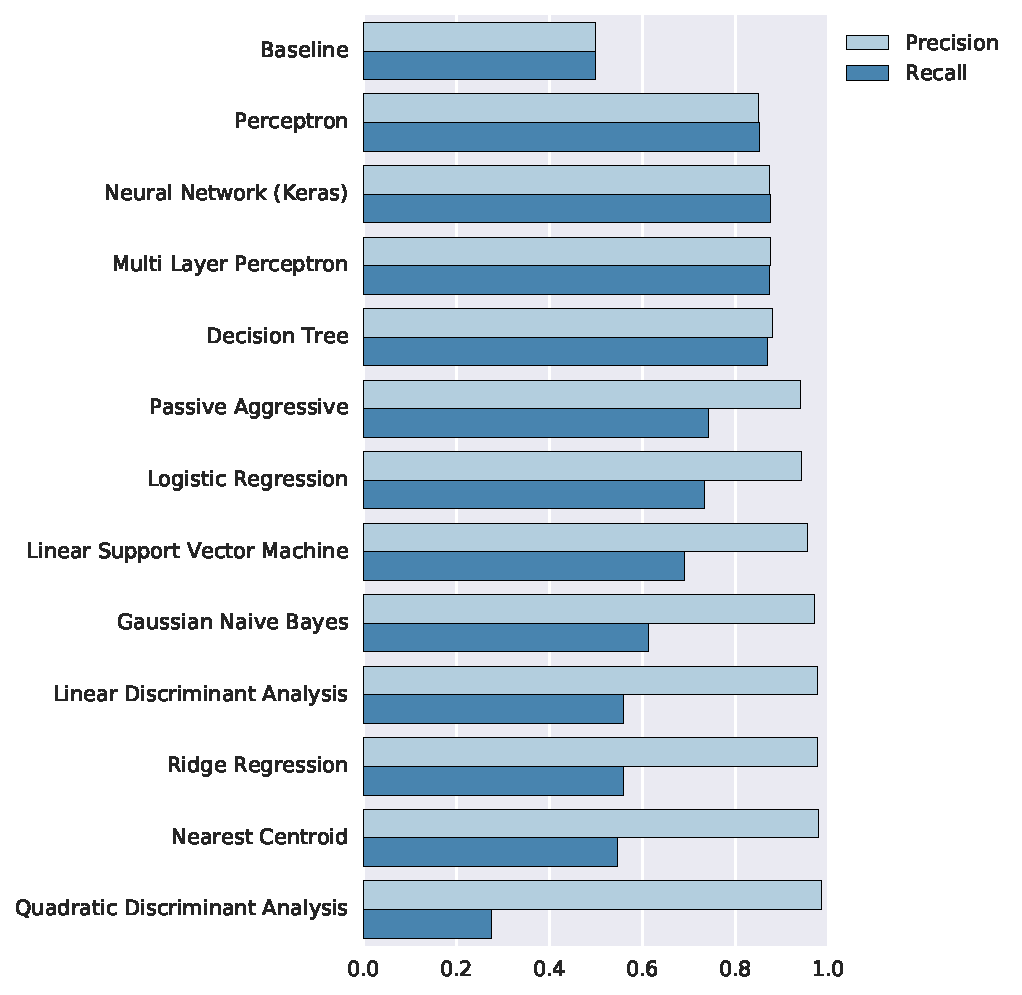
\includegraphics[width=0.95\textwidth]{classifier-comparison2.pdf}
%\caption[Precision and recall scores for the chosen algorithms]{Precision and recall scores for the chosen algorithms, sorted by precision.}\label{fig:classifier_comparison}
%\end{figure}

\begin{figure}[tb]%
\centering
\tikzsetnextfilename{barchart}
\begin{tikzpicture}
  \begin{axis}[
      table/col sep=semicolon,
      xbar=0pt, xmin=0, xmax=1,
      xlabel=Score,
      yticklabels from table={chapter_design/10f-results.csv}{name},
      %yticklabel style={text height=1.5ex},
      ytick=data,
      width=0.6\textwidth,
      y=0.8cm,
      enlarge y limits={abs=0.6},
      bar width=7pt,
      /pgf/number format/fixed,
      axis lines*=left,
      xmajorgrids=true,
      legend entries={Recall, Precision},
      legend style={draw=none},
      reverse legend, area legend,
      legend style={at={(1,1.01)},anchor=south east}
    ]
    \addplot [fill=color1!20!white] table [y expr=-\coordindex, x=recall] {chapter_design/10f-results.csv};
    \addplot [fill=color1!70!white] table [y expr=-\coordindex, x=precision] {chapter_design/10f-results.csv};

  \end{axis}
\end{tikzpicture}
\caption[Precision and recall scores for the chosen algorithms]{Precision and recall scores for the tested algorithms, sorted by precision}\label{fig:classifier_comparison}%
\end{figure}

% \begin{table}[tbp]
% \centering
% \begin{tabular}{@{}lp{.75\textwidth}@{}}
% \toprule
% \textbf{Classifier} & \textbf{Result} \\
% \midrule
% Baseline           &  DummyClassifier()                \\
% Nearest Neighbors  &  KNeighborsClassifier(3)          \\
% Linear SVM         &  SVC(kernel="linear", C=0.025)    \\
% RBF SVM            &  SVC(gamma=2, C=1)                \\
% Gaussian Process   &  GaussianProcessClassifier        \\
% Decision Tree      &  DecisionTreeClassifier           \\
% Random Forest      &  RandomForestClassifier           \\
% Neural Net         &  MLPClassifier, KerasClassifier   \\
% AdaBoost           &  AdaBoostClassifier()             \\
% Naive Bayes        &  GaussianNB()                     \\
% QDA                &  QuadraticDiscriminantAnalysis()  \\
% \bottomrule
% \end{tabular}
% \caption[Classifiers]{Classifiers}%
% \label{tab:classifiers}
% \end{table}

% \subsection{Classifier Parameter Optimization}
% To attempt to further increase the performance of the chosen classifier, we optimize its parameters. The \emph{nearest centroid} implementation in the \emph{scikit-learn} library only has two parameters, so we use grid search to explore possible parameter combinations, as the parameter space is small.

% Searching the parameter space reveals that the default parameters, with a euclidean distance metric, and no feature shrink threshold specified, gives the best performance.


\section[UI]{User Interface}
% Første parameter i [] er tekst i header. {} er i indholdsfortegnelsen.

% Slide med emneoverskrift.
\begin{frame}
  \frametitle{}
  \begin{center}
    {\Huge User Interface}
  \end{center}
\end{frame}
\note{
  \begin{itemize}
		\item Notes...
  \end{itemize}
}

% Normal slide:
\begin{frame}
    \frametitle{Some Example Title}
    \framesubtitle{Some example subtitle}
    \centering
    Some text, content, etc.
\end{frame}
\note{
	\begin{itemize}
    \item Notes here...
	\end{itemize}
}
